\section{Dependency}
\label{sec:dependency}

\begin{figure}[h!] 
	\centering
	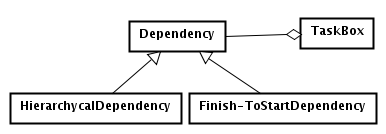
\includegraphics[width=0.5\textwidth]{../DependencyDetail.png}
	\caption{dependencies}
	\label{fig:dependencies} 
\end{figure}

\emph{Dependency} modella il tipo di dipendenze che possiamo rappresentare in
un \emph{Chart}. Per implementare la specifica abbiamo bisogno di incapsulare
queste varianti:\footnote{dire in quali Chart vengono utilizzate}
\begin{itemize}
  \item \emph{Finish-ToStartDependency}: siano $a, b$ due \emph{Task} tali
  che $b$ non pu\`o iniziare finch\'e $a$ non sia completato. Questa relazione
  \`e catturata da questa specializzazione.
  \item \emph{HierarchycalDependency}: siano $a, b_{i}$ con $i= 1,\ldots,n \in
  N$, \emph{Task}s tali che $a$ \`e scoposto in $b_{i}$ \emph{Task}. Questa
  relazione \`e catturata da questa specializzazione.
\end{itemize}